\section{Set galvanometrů se~zrcátky} \label{sec:my-galvos}
\subsection{Výběr skeneru}
Pro tuto práci byl vybrán galvanometrový skener, protože je~nejdostupnější a~protože potenciálním uživatelům nejlépe představí technologii.

Oproti hranolovým skenerům jim tožiž dává více možností, jak s paprskem pohybovat.
Můžou se~rozhodnout, že jej využijí jako hranolový skener, pokud nahrají soubor procházející promítací plochu po~řádcích.

Oproti dalším typům skenerů je~názornější, ostatní typy skenerů jsou totiž příliš malé a~není na~nich vidět princip funkce nebo je~jejich fungování nadmíru abstraktní a~těžko pochopitelné.

\subsection{Zapojení galvanometrového setu}
Samotné galvanometry jsou zapojeny do~řídící desky, která s nimi byla zakoupena, ta je vidět na obrázku~\ref{fig:hw_galvoboard}.

Řídící deska požaduje symetrický zdroj napětí 15~V, tzn. $+15$~V a~$-15$~V a~samozřejmě připojení k zemi. Také přijímá dva bipolární diferenciální analogové signály s~rozsahem diferenciálního napětí $-10$~V až $+10$~V. Každý signál udává vychýlení jednoho ze~dvou galvanometrů, což obvykle znamená výslednou pozici laserového paprsku v~osách X~a~Y.

\begin{figure}[htb]
  \centering
  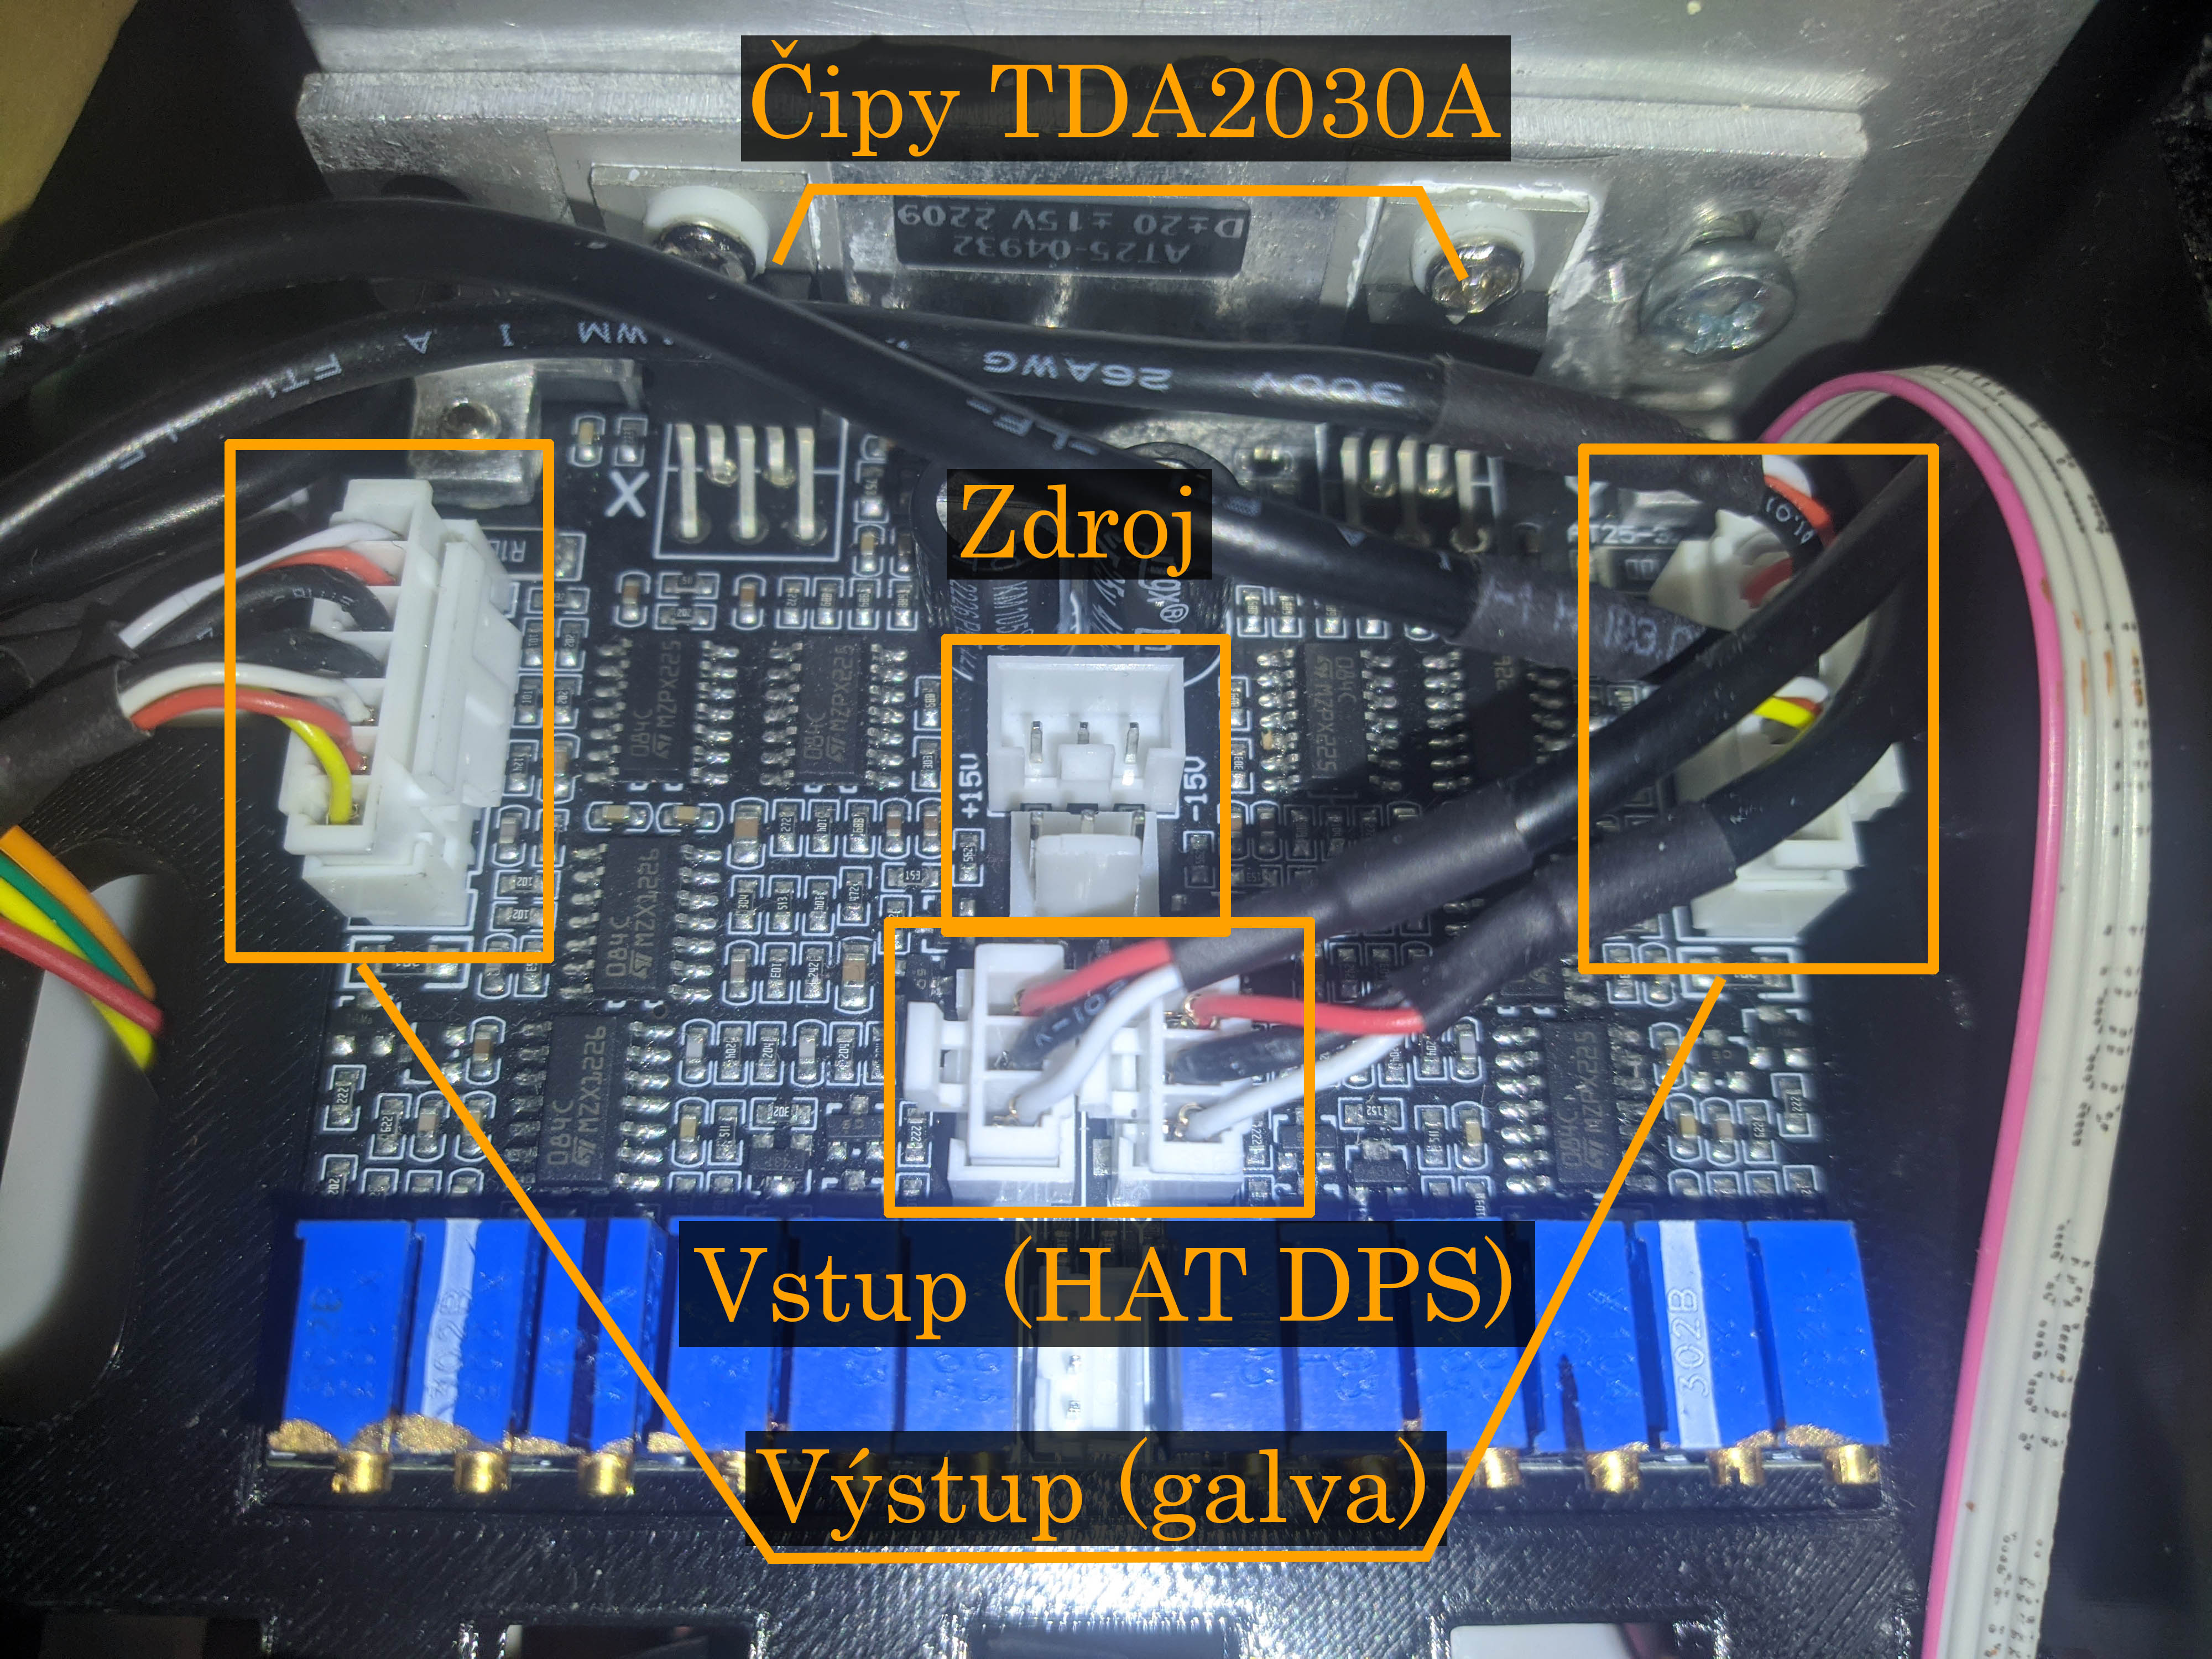
\includegraphics[width=1\textwidth]{img/hw_galvoboard.jpg}
  \caption{\label{fig:hw_galvoboard} Řídící deska galvanometrů s vyznačenými konektory a hřejícími čipy}
\end{figure}

\subsection{Bipolární diferenciální analogový signál}
Diferenciální signál je~signál přenášený dvěma vodiči, každý z~nich přenáší stejný signál, jen s~opačnou polaritou. Kontakt označený $(+)$ je~považován za~nosič základního signálu, zatímco kontakt označený $(-)$ je~považován za~nosič invertovaného signálu. Výsledné diferenciální napětí je~napětí na~základním nosiči vůči napětí na~obráceném nosiči, tzn.~$V_{dif} = V_{(+)} - V_{(-)}$.~\cite{ilda-signal-spec}

Bipolární signál znamená, že na~napětí každém z~kontaktů $(+)$ a~$(-)$ může dosahovat kladných i~záporných hodnot~\cite{ilda-signal-spec}.

Tudíž cheme-li disáhnout diferenciálního napětí $+10~V$, musí mít základní signál napětí $+5~V$ a~obrácený signál $-5~V$. Záporné diferenciální napětí bude ve~chvíli, kdy je~napětí základního signálu záporné a~napětí obráceného signálu kladné.

\subsection{Zahřívání čipů řídící desky galvanometrů} \label{sec:galvoboard-chips-heating-up}
Dva z~čipů na~řídící desce se při chodu systému výrazně zahřívájí. Na~tyto čipy je naštěstí už od~výroby desky připevněna malá hliníková destička. Ta~má sloužit jako chladič, ale i~s ní se~čipy v~otevřeném prostoru zahřívají na~teploty blízké 60~\degree{}C.
Dva zmíněné čipy jsou čipy TDA2030A od~firmy STMicroelectronics. Ty~by~měly dle datasheetu vydržet až 150~\degree{}C, ale dá se~předpokládat, že v~uzavřeném pouzdru budou čipy dosahovat vyšších teplot, než v~otevřeném prostoru. I~kdyby nedosáhly pro sebe kritických 150~\degree{}C, rozhodně není žádoucí, aby uvnitř projektoru desky dosahovaly vysokých teplot.

I proto byl do~projektoru zabudován chladič. Více o~způsobu jeho připevnění a~distribuci chlazení mezi ostatní komponenty se~dočtete v~kapitole~\ref{sec:krabick-design-priorities}.
